% compiler : XeLaTex
% Bib type : BibLaTex using Biber


% 文档类型
\documentclass[11pt, twoside,openright]{ctexbook}

% 论文信息


%\ProvidesPackage{nuaaThesisInfos}[2025/5/02 1.0 Thesis package]

%论文信息

\newcommand{\nuaaMasterOrDoctor}{硕}
\newcommand{\nuaaDegreeEn}{Master of Academic}

\newcommand{\nuaaBookClassNum}{V123.45}
\newcommand{\nuaaThesisid}{123456789}
\newcommand{\nuaaSubjectNum}{123456}

\newcommand{\nuaaName}{南京航空航天大学}
\newcommand{\nuaaNameEn}{Nanjing University of Aeronautics and Astronautics}
\newcommand{\nuaaPageHeader}{南京航空航天大学\nuaaMasterOrDoctor 士学位论文}

\newcommand{\nuaaTitle}{标题标题标题标题标题\\标题太长,手动换行}
\newcommand{\nuaaTitleHead}{用于页眉的标题}
\newcommand{\nuaaTitleEn}{
	English Tilte here
	}
\newcommand{\nuaaAuthorName}{姓名}
\newcommand{\nuaaAuthorNameEn}{english name}
\newcommand{\nuaaMajor}{专业名称}
\newcommand{\nuaaMajorEn}{Major English }
\newcommand{\nuaaInterests}{研究方向}
\newcommand{\nuaaBigBossName}{导师姓名\quad 教授}
\newcommand{\nuaaBigBossNameEn}{mentor name}

\newcommand{\nuaaCollege}{XXX学院}
\newcommand{\nuaaCollegeEn}{College of LaTeX Writting}

\newcommand{\nuaaDate}{一九五二年十月}
\newcommand{\nuaaDateEn}{Oct, 1952}



%% Cover ( anonymous )
% 用于查重的封面、也可作为模板,隐藏个人信息

%\ProvidesPackage{nuaaThesisInfos}[2025/5/02 1.0 Thesis package]

%论文信息

\newcommand{\nuaaMasterOrDoctor}{硕}
\newcommand{\nuaaDegreeEn}{Master of Academic}

\newcommand{\nuaaBookClassNum}{V123.45}
\newcommand{\nuaaThesisid}{123456789}
\newcommand{\nuaaSubjectNum}{123456}

\newcommand{\nuaaName}{*}
\newcommand{\nuaaNameEn}{*********** University}
\newcommand{\nuaaPageHeader}{*\nuaaMasterOrDoctor 士学位论文}

\newcommand{\nuaaTitle}{标题标题标题标题\\标题太长手动换行}
\newcommand{\nuaaTitleHead}{用于页眉的标题}
\newcommand{\nuaaTitleEn}{
	English Tilte here
}
\newcommand{\nuaaAuthorName}{*}
\newcommand{\nuaaAuthorNameEn}{*}
\newcommand{\nuaaMajor}{专业名称}
\newcommand{\nuaaMajorEn}{Major English }
\newcommand{\nuaaInterests}{研究方向}
\newcommand{\nuaaBigBossName}{*}
\newcommand{\nuaaBigBossNameEn}{*}

\newcommand{\nuaaCollege}{*}
\newcommand{\nuaaCollegeEn}{* College}

\newcommand{\nuaaDate}{二〇二五年一月}
\newcommand{\nuaaDateEn}{January, 2025}


 % 查重时请取消注释,并将上一行注释取消

% NUAA样式自定义宏包
\usepackage{Settings/nuaaThesisStyle}

% 参考文献文件路径
\addbibresource{References/references.bib} % 主文档中设置参考文献路径

% 文档开始
\begin{document}
	
	% 中文封面、英文封面、签署页
	\begingroup
	
% 封面
	
% 辅助宏
\newcolumntype{J}{>{\raggedright\arraybackslash}X}
\newcolumntype{L}{>{\RaggedRight\hangafter=1\hangindent=0em}X}
\newcommand{\mysep}{\hspace{5.33pt}}
\newcommand\covertable[2][7cm]{\makebox[#1][l]{#2}} 
\newcommand\xiahuabox[2][4cm]{\underline{\makebox[#1][c]{#2}}} 

\begin{titlepage}
	
	%----------------------中文封面----------------------
	
	\begin{flushleft}
		中图分类号:\nuaaBookClassNum \hfill 论文编号:\nuaaThesisid \\
		学科分类号:\nuaaSubjectNum
	\end{flushleft}
	
	\centering
	\vspace*{1cm}
	
	{\songti\zihao{0} \nuaaMasterOrDoctor 士学位论文 \par}
	
	\vspace{1.5cm}
	
	{\heiti\zihao{1} \nuaaTitle \par}
		
	\vspace{2cm}

	\zihao{3}
	{
		\songti
		\makebox[2.9cm][s]{研究生姓名}\makebox[1.7cm][s]{}\covertable[5cm]{\nuaaAuthorName}\\
		\makebox[2.9cm][s]{学科、专业}\makebox[1.7cm][s]{}\covertable[5cm]{\nuaaMajor}\\
		\makebox[2.9cm][s]{研究方向}\makebox[1.7cm][s]{}\covertable[5cm]{\nuaaInterests}\\
		\makebox[2.9cm][s]{指导教师}\makebox[1.7cm][s]{}\covertable[5cm]{\nuaaBigBossName}\\
	}
	
	\vfill

	{\minijianqi\zihao{2}\nuaaName \par}% 迷你简启体 这玩意儿得单独下载,一般电脑没有装
	\vspace{0.3cm}
	{\kaishu\zihao{-2} 研究生院\quad \nuaaCollege \par}
	\vspace{0.1cm}
	{\kaishu\zihao{3} \nuaaDate \par} 
	
	%空白
	\clearpage
	\phantom{s}
	\thispagestyle{empty}
	\clearpage


	%----------------------英文封面----------------------
	\newpage
	\thispagestyle{empty}
	\setmainfont{Times New Roman}
	
	\vspace*{-10pt}
	\zihao{4}{\nuaaNameEn \par
	\nuaaCollegeEn \par}
	
	\vspace*{30pt}
	
	\setstretch{1.2}\zihao{2}{\bfseries \nuaaTitleEn \par}
	
	\vspace*{1.35cm}
	
	\setstretch{1.6}\zihao{4}A Thesis in \par
	\nuaaMajorEn  \par
	\vspace*{4pt}
	by\par
	\nuaaAuthorNameEn \par
	\vspace*{2pt}
	Advised by \par
	\vspace*{6pt}
	Prof. \nuaaBigBossNameEn \par
	\vspace*{10pt}
	Submitted in Partial Fulfillment\par\par
	\vspace*{8pt}
	of the Requirements\par
	\vspace*{6pt}
	for the Degree of\par
	\vspace*{10pt}
	\nuaaDegreeEn \par
	\vspace*{35pt}
	\nuaaDateEn
	
	
	%空白页
	\clearpage
	\phantom{s}
	\thispagestyle{empty}
	\clearpage
	
	
	%----------------------承诺书签署页----------------------
	\newpage
	\thispagestyle{empty}
	
	\vspace*{-10pt}
	
	\zihao{2}{承诺书}\par
	
	\vspace*{1cm}
	
	\zihao{3}\justifying{本人声明所呈交的\nuaaMasterOrDoctor 士学位论文是本人在导师指导下进行的研究工作及取得的研究成果。除了文中特别加以标注和致谢的地方外,论文中不包含其他人已经发表或撰写过的研究成果,也不包含为获得\nuaaName 或其他教育机构的学位或证书而使用过的材料。\par
	本人授权\nuaaName 可以将学位论文的全部或部分内容编入有关数据库进行检索,可以采用影印、缩印或扫描等复制手段保存、汇编学位论文。\par
	(保密的学位论文在解密后适用本承诺书)\par
	}
	
	\vspace*{4.3cm}
	
	\flushright{\zihao{3} 
		\songti
		\makebox[2.3cm][s]{作者签名}:\xiahuabox[3.2cm]{}\\
		\makebox[2.3cm][s]{日期}:\xiahuabox[3.2cm]{}\\
	}

	%空白页
	\clearpage
	\phantom{s}
	\thispagestyle{empty}
	\clearpage
	
\end{titlepage}
	\endgroup	
	
	% 前置部分
	\frontmatter
	\pagenumbering{roman} % 小罗马字页码
	
	% 中英文摘要
	% 摘要


%----------------------中文摘要----------------------
\chapter*{\heiti\zihao{-3} 摘\quad 要}
%\addcontentsline{toc}{chapter}{摘要} 
{
	\songti\zihao{5}

这里是摘要这里是摘要这里是摘要这里是摘要这里是摘要这里是摘要这里是摘要这里是摘要这里是摘要这里是摘要这里是摘要这里是摘要这里是摘要这里是摘要这里是摘要这里是摘要这里是摘要这里是摘要这里是摘要这里是摘要这里是摘要这里是摘要这里是摘要这里是摘要这里是摘要这里是摘要这里是摘要

这里是摘要这里是摘要这里是摘要这里是摘要这里是摘要这里是摘要这里是摘要这里是摘要这里是摘要这里是摘要这里是摘要这里是摘要这里是摘要这里是摘要这里是摘要这里是摘要这里是摘要这里是摘要这里是摘要这里是摘要这里是摘要这里是摘要这里是摘要这里是摘要这里是摘要这里是摘要这里是摘要

这里是摘要这里是摘要这里是摘要这里是摘要这里是摘要这里是摘要这里是摘要这里是摘要这里是摘要这里是摘要这里是摘要这里是摘要这里是摘要这里是摘要这里是摘要这里是摘要这里是摘要这里是摘要这里是摘要这里是摘要这里是摘要这里是摘要这里是摘要这里是摘要这里是摘要这里是摘要这里是摘要

这里是摘要这里是摘要这里是摘要这里是摘要这里是摘要这里是摘要这里是摘要这里是摘要这里是摘要这里是摘要这里是摘要这里是摘要这里是摘要这里是摘要这里是摘要这里是摘要这里是摘要这里是摘要这里是摘要这里是摘要这里是摘要这里是摘要这里是摘要这里是摘要这里是摘要这里是摘要这里是摘要
这里是摘要这里是摘要这里是摘要这里是摘要这里是摘要这里是摘要这里是摘要这里是摘要这里是摘要这里是摘要这里是摘要这里是摘要这里是摘要这里是摘要这里是摘要这里是摘要这里是摘要这里是摘要

}
\vspace*{2.5cm}
{\noindent\bfseries 关键词 :}  
关键词;关键词;关键词;关键词;关键词;关键词


%----------------------英文摘要----------------------


\chapter*{\setmainfont{Times New Roman}\zihao{4}\bfseries ABSTRACT}
%\addcontentsline{toc}{chapter}{ABSTRACT}%添加到目录
{
\setmainfont{Times New Roman}
\zihao{5}

English abstract English abstract English abstract English abstract English abstract English abstract English abstract English abstract English abstract English abstract 

English abstract English abstract English abstract English abstract English abstract English abstract English abstract English abstract English abstract English abstract English abstract English abstract English abstract English abstract English abstract English abstract English abstract English abstract English abstract English abstract English abstract English abstract English abstract English abstract English abstract English abstract English abstract English abstract English abstract English abstract English abstract English abstract English abstract English abstract English abstract English abstract English abstract English abstract English abstract English abstract 

English abstract English abstract English abstract English abstract English abstract English abstract English abstract English abstract English abstract English abstract English abstract English abstract English abstract English abstract English abstract English abstract English abstract English abstract English abstract English abstract English abstract English abstract English abstract English abstract English abstract English abstract English abstract English abstract English abstract English abstract English abstract English abstract English abstract English abstract English abstract English abstract English abstract English abstract English abstract English abstract English abstract English abstract English abstract English abstract English abstract English abstract English abstract English abstract English abstract English abstract 

English abstract English abstract English abstract English abstract English abstract English abstract English abstract English abstract English abstract English abstract English abstract English abstract English abstract English abstract English abstract English abstract English abstract English abstract English abstract English abstract English abstract English abstract English abstract English abstract English abstract English abstract English abstract English abstract English abstract English abstract English abstract English abstract English abstract English abstract English abstract English abstract English abstract English abstract English abstract English abstract 

English abstract English abstract English abstract English abstract English abstract English abstract English abstract English abstract English abstract English abstract English abstract English abstract 

}
\vspace*{2.5cm}
{\noindent\bfseries Keywords:}
Keywords, Keywords, Keywords, Keywords, Keywords



	
	% 目录
	\cleardoublepage % 确保从右侧页开始
	\tableofcontents
	
	% 图表清单
	\cleardoublepage % 确保从右侧页开始
	\phantomsection %\addcontentsline 前需使用 \phantomsection 以正确设置超链接位置。
%	\addcontentsline{toc}{chapter}{图表清单} 
	\begingroup
	\renewcommand*{\addvspace}[1]{} % 去除图表目录中每章之间的间隔
		\listoffigures
		\listoftables
	\endgroup
 
	
	%注释表、缩略词
	\cleardoublepage % 确保从右侧页开始
	

%----------------------注释表----------------------

\newpage
\vspace*{-2pt}
{\centering\heiti\zihao{-3}注释表\par}
\phantomsection %\addcontentsline 前需使用 \phantomsection 以正确设置超链接位置。
%\addcontentsline{toc}{chapter}{注释表} 
%
\LTXtable{0.9\textwidth}{Others/symbol}

%----------------------缩略词----------------------
\newpage
\vspace*{-2pt}
{\centering\heiti\zihao{-3}缩略词\par}
\phantomsection %\addcontentsline 前需使用 \phantomsection 以正确设置超链接位置。
%\addcontentsline{toc}{chapter}{缩略词} 

\LTXtable{0.9\textwidth}{Others/abbreviation}

	% 正文部分
	\mainmatter
	\pagenumbering{arabic} %罗马数字页码
	
	

\chapter{绪论}

\section{背景和意义}


\section{论文研究内容及章节安排}





	\chapter{常用}

\section{图片}

\subsection{单图居中}
如图~\ref{fig::graphexample}所示
\begin{figure}[htbp]
	\centering
	
\includegraphics[width = 0.9\textwidth]{./Graphs/example/example.jpeg} 
	\caption{单栏居中图片}
	\label{fig::graphexample} 
\end{figure}
\subsection{双列跨页子图}

\begin{figure}[!ht] \centering
	\begin{subfigure}[b]{0.49\textwidth}\centering
		
\includegraphics[width=\textwidth]{./Graphs/example/example.jpeg}
		\caption{sub1}\label{subf::sub1}
	\end{subfigure}\hfill % 插入间隔
	\begin{subfigure}[b]{0.49\textwidth}\centering
		
\includegraphics[width=\textwidth]{./Graphs/example/example.jpeg}
		\caption{sub2}\label{subf::sub2}
	\end{subfigure}
\end{figure}
\begin{figure}[!ht]\ContinuedFloat \centering
	\begin{subfigure}[b]{0.49\textwidth}\centering
		
\includegraphics[width=\textwidth]{./Graphs/example/example.jpeg}
		\caption{sub3}\label{subf::sub3}
	\end{subfigure}\hfill % 插入间隔
	\begin{subfigure}[b]{0.49\textwidth}\centering
		
\includegraphics[width=\textwidth]{./Graphs/example/example.jpeg}
		\caption{sub4}\label{subf::sub4}
	\end{subfigure}
\end{figure}
\begin{figure}[!ht]\ContinuedFloat \centering
	\begin{subfigure}[b]{0.49\textwidth}\centering
		
\includegraphics[width=\textwidth]{./Graphs/example/example.jpeg}
		\caption{sub5}\label{subf::sub5}
	\end{subfigure}\hfill % 插入间隔
	\begin{subfigure}[b]{0.49\textwidth}\centering
		
\includegraphics[width=\textwidth]{./Graphs/example/example.jpeg}
		\caption{sub6}\label{subf::sub6}
	\end{subfigure}
\end{figure}
\begin{figure}[!ht]\ContinuedFloat \centering
	\begin{subfigure}[b]{0.49\textwidth}\centering
		
\includegraphics[width=\textwidth]{./Graphs/example/example.jpeg}
		\caption{sub7}\label{subf::sub7}
	\end{subfigure}\hfill % 插入间隔
	\begin{subfigure}[b]{0.49\textwidth}\centering
		
\includegraphics[width=\textwidth]{./Graphs/example/example.jpeg}
		\caption{sub8}\label{subf::sub8}
	\end{subfigure}
\end{figure}
\begin{figure}[!ht]\ContinuedFloat \centering
	\begin{subfigure}[b]{0.49\textwidth}\centering
		
\includegraphics[width=\textwidth]{./Graphs/example/example.jpeg}
		\caption{sub9}\label{subf::sub9}
	\end{subfigure}\hfill % 插入间隔
	\begin{subfigure}[b]{0.49\textwidth}\centering
		
\includegraphics[width=\textwidth]{./Graphs/example/example.jpeg}
		\caption{sub10}\label{subf::sub10}
	\end{subfigure}
\end{figure}
\begin{figure}[!ht]\ContinuedFloat \centering
	\begin{subfigure}[b]{0.7\textwidth}\centering
		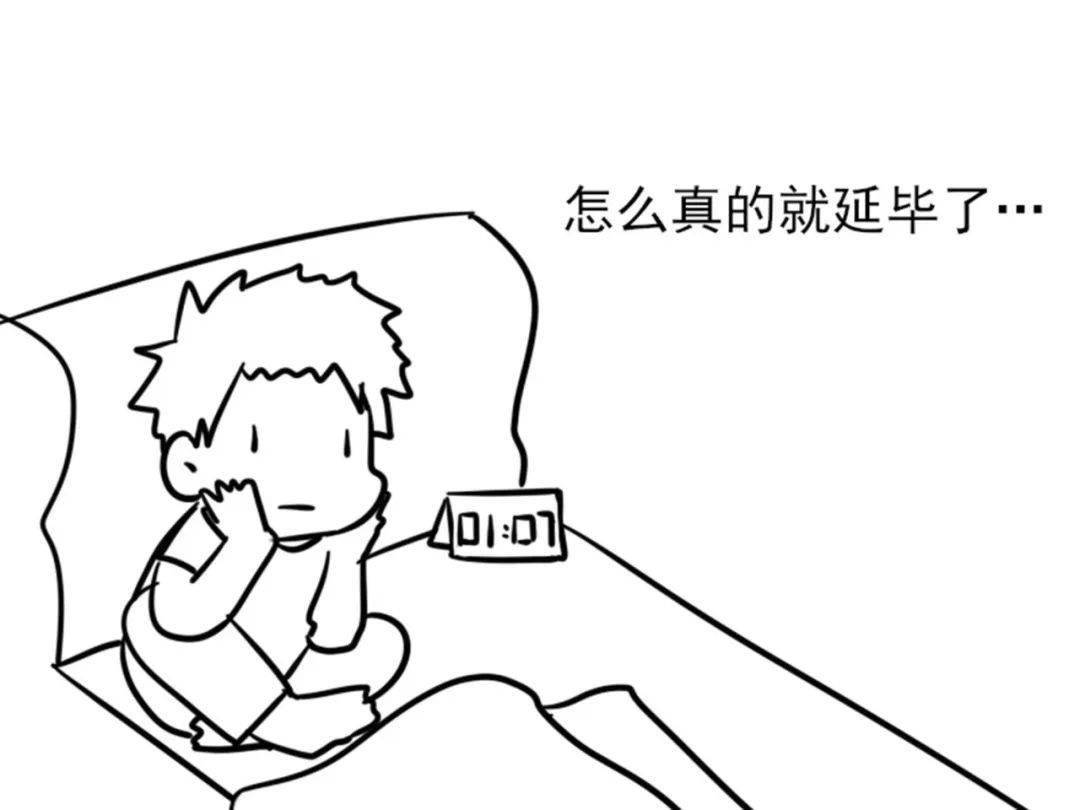
\includegraphics[width=\textwidth]{./Graphs/example/example_2.jpeg}
		\caption{sub11}\label{subf::sub11}
	\end{subfigure}
	\caption{双列跨页子图}
	\label{fig::dual_col_subfigs}
\end{figure}
\FloatBarrier


图~\ref{fig::dual_col_subfigs}\subref{subf::sub1}和图~\ref{fig::dual_col_subfigs}\subref{subf::sub3}分别为XXXXXXXXXXXXXX。

\section{表格}

\subsection{简单表格}

	如表~\ref{tab::table_demo_1}所示。
	\begin{table}[htbp]
		\renewcommand{\arraystretch}{1.5}
		\centering
		\zihao{5}
		\caption{XXXXXXXXXXXXX表}
		\begin{tabular}{c c p{10pt} c c} 
			\toprule % 表头上方线
			表头 & 表头 	&& 表头 & 表头\\ 
			\midrule % 表头与内容间线
			XXX& XXX &&  XXX & XXX\\ 
			XXX& XXX	 && XXX & XXX \\
			XXX& XXX 	 && XXX & XXX \\
			XXX & XXX	 && XXX & XXX \\
			XXX& XXX	 && XXX & XXX \\
			XXX & XXX	 && XXX & XXX \\
			XXX  & 	XXX && XXX & XXX \\
			XXX &  XXX	 && XXX & XXX \\
	 		XXX  & XXX	 && XXX &  XXX\\
	 		XXX  & XXX	 && XXX &  XXX\\
	 		XXX	& XXX	 && XXX &  XXX\\
	 		XXX    & XXX	 && XXX & XXX\\
			\bottomrule % 表底线
		\end{tabular}
		\label{tab::table_demo_1}
	\end{table}
	
	\subsection{跨页表格处理}
	
	见符号表
	
\section{公式}
\subsection{行内公式}

行内$a = b + c$公式


\subsection{单行公式}

如式\ref{eq::example}所示。

\begin{equation}\label{eq::example}
	A=\sqrt{AAAA\left(1-\left(\dfrac{AAAA_{AAAA}}{AAAA}\right)^{\dfrac{A^{\prime}-1}{A^{\prime}}}\right)} 
\end{equation}

\subsection{多行公式}

\begin{equation}
	\left\{\begin{array}{l}
		A = \alpha  \\
		B = \beta \\
		O = \omega
	\end{array}\right.
\end{equation}


\subsection{条件公式}
使用\&符号对齐。
\begin{equation}
	\begin{cases}
		case\quad a & , A>1  
		\\ case\quad b & , B>1 
		\\ case\quad c & , C<1
	\end{cases}
\end{equation}
\subsection{矩阵}

\begin{equation}\label{eq::example_tab}
	A=
	\begin{bmatrix}
		0 & 0 & 2.243 & 0 & -0.2575 & 0\\
		0.0021 & -3.771 & 0 & -0.3055 & 0.0002 & 0.1823\\
		0 & 0 & 0 & 0 & -0.9035 &0 \\
		0 & 0 & 0 & -7.8760 & 0 & 4.6860\\
		0 & 0 & 0 & 0 & 1.99 & 0\\
		-12.09 & 0 & 0 & -0.0519 & 0.0004 &-0.0322
	\end{bmatrix}
\end{equation}


\section{列表项}

\subsection{带编号}
	列表项
	
	\begin{enumerate}[label=(\arabic*),listparindent=2em,left = 2em,topsep = 0pt,itemsep = 0pt,parsep= 0pt,partopsep=0pt]
		\item 列表内容列表内容列表内容
		\item 列表内容列表内容列表内容
		\item 列表内容列表内容列表内容
		\item 列表内容列表内容列表内容
		\item 列表内容列表内容列表内容
		\item 列表内容列表内容列表内容
	\end{enumerate}
	

\section{参考文献引用}

\subsection{角标}

某某\cite{ref_thesis}XXXXXXXXXXXX,某某\cite{ref_book}XXXXXXXXXXXX。

\subsection{强调}

根据文献中\parencite{ref_article}的


















	\chapter{第三章}


	\chapter{第四章}











	\chapter{第五章}




	\chapter{总结与展望}

\section{本文工作总结}
	本文工作总结本文工作总结本文工作总结本文工作总结本文工作总结本文工作总结本文工作总结本文工作总结本文工作总结本文工作总结本文工作总结本文工作总结本文工作总结本文工作总结本文工作总结本文工作总结本文工作总结本文工作总结本文工作总结本文工作总结本文工作总结本文工作总结本文工作总结本文工作总结本文工作总结本文工作总结本文工作总结本文工作总结.
	
%\section{创新点}
%本文创新点如下:
%(1)
%(2)
%(3)
\section{未来工作展望}

未来工作展望未来工作展望未来工作展望未来工作展望未来工作展望未来工作展望未来工作展望未来工作展望未来工作展望未来工作展望未来工作展望未来工作展望未来工作展望未来工作展望.






	
	% 参考文献
	\cleardoublepage % 确保从右侧页开始
	\printbibliography
	\addcontentsline{toc}{chapter}{参考文献} 
	\nocite{*} %列出未引用的参考文献
	
	% 致谢
	

%----------------------致谢----------------------
\chapter*{致谢}
\addcontentsline{toc}{chapter}{致谢} 

感谢。

生僻字处理:{\CJKfontspec{simsun.ttc}旻}、{\CJKfontspec{simsun.ttc}宬}。


\vspace{2cm}
\begin{flushright}
	\begin{tabular}{c}
	
\includegraphics[width=2cm]{./Settings/signature.png}\\
	二零二五年一月于XXXX
	\end{tabular}
\end{flushright}



%我感谢天地,我感谢父母,我是罪人,我危害人间,我辜负苍生,我愿抛开一切,消除我名利权力,舍弃金钱物质,归于真我‌;我感谢天地,我感谢父母,我是罪人,我危害人间,我辜负苍生,我愿抛开一切,消除我名利权力,舍弃金钱物质,归于真我‌;我感谢天地,我感谢父母,我是罪人,我危害人间,我辜负苍生,我愿抛开一切,消除我名利权力,舍弃金钱物质,归于真我‌;我感谢天地,我感谢父母,我是罪人,我危害人间,我辜负苍生,我愿抛开一切,消除我名利权力,舍弃金钱物质,归于真我‌;我感谢天地,我感谢父母,我是罪人,我危害人间,我辜负苍生,我愿抛开一切,消除我名利权力,舍弃金钱物质,归于真我‌;我感谢天地,我感谢父母,我是罪人,我危害人间,我辜负苍生,我愿抛开一切,消除我名利权力,舍弃金钱物质,归于真我‌;我感谢天地,我感谢父母,我是罪人,我危害人间,我辜负苍生,我愿抛开一切,消除我名利权力,舍弃金钱物质,归于真我‌;我感谢天地,我感谢父母,我是罪人,我危害人间,我辜负苍生,我愿抛开一切,消除我名利权力,舍弃金钱物质,归于真我‌;我感谢天地,我感谢父母,我是罪人,我危害人间,我辜负苍生,我愿抛开一切,消除我名利权力,舍弃金钱物质,归于真我‌;我感谢天地,我感谢父母,我是罪人,我危害人间,我辜负苍生,我愿抛开一切,消除我名利权力,舍弃金钱物质,归于真我‌;我感谢天地,我感谢父母,我是罪人,我危害人间,我辜负苍生,我愿抛开一切,消除我名利权力,舍弃金钱物质,归于真我‌;我感谢天地,我感谢父母,我是罪人,我危害人间,我辜负苍生,我愿抛开一切,消除我名利权力,舍弃金钱物质,归于真我‌;我感谢天地,我感谢父母,我是罪人,我危害人间,我辜负苍生,我愿抛开一切,消除我名利权力,舍弃金钱物质,归于真我‌;我感谢天地,我感谢父母,我是罪人,我危害人间,我辜负苍生,我愿抛开一切,消除我名利权力,舍弃金钱物质,归于真我‌;\par
%我感谢天地,我感谢父母,我是罪人,我危害人间,我辜负苍生,我愿抛开一切,消除我名利权力,舍弃金钱物质,归于真我‌;我感谢天地,我感谢父母,我是罪人,我危害人间,我辜负苍生,我愿抛开一切,消除我名利权力,舍弃金钱物质,归于真我‌;
	
	% 在学期间的研究成果及发表的学术论文
	
%----------------------在学期间的研究成果及发表的学术论文----------------------
\chapter*{在学期间的研究成果及发表的学术论文}
\addcontentsline{toc}{chapter}{在学期间的研究成果及发表的学术论文} 

\zihao{5}{\heiti \noindent 攻读\nuaaMasterOrDoctor 士学位期间发表(录用)论文情况}\par

\begin{enumerate}[itemsep = -5pt, left = 0pt]
	\item \textbf{XXX},XX,XX,等.~XXXXXXXXXXXXXXXXXXXXXXXXXXXXXXXX[J].~XXXXXXXXXXXX学报.(已录用,中文核心)
%	\item \textbf{XXX},XX,XX,等.~XXXXXXXXXXXXXXXXXXXXXXXXXXXXXXXX[J].~XXXXXXXXXXXX学报.(已录用,中文核心)
\end{enumerate}

\vspace*{2cm}
\zihao{5}\heiti{\noindent 攻读\nuaaMasterOrDoctor 士学位期间专利发表情况 }\par
\begin{enumerate}[itemsep = -5pt, left = 0pt]
	\item 
\end{enumerate}

\vspace*{2cm}

\zihao{5}{\heiti \noindent 攻读\nuaaMasterOrDoctor 士学位期间参加科研项目情况}\par

\begin{enumerate}[itemsep = -5pt, left = 0pt]
	\item 项目项目项目项目项目项目项目,XXX项目,主要参与人;(已结题)
\end{enumerate}


	
%	% 附录
%	\appendix
%	\songti
	
%	\chapter*{附录\quad 代码}
%	\addcontentsline{toc}{chapter}{附录\quad 代码} 
%	附录内容……
	
%	\chapter*{附录\quad 图表}
%	\addcontentsline{toc}{chapter}{附录\quad 图表} 
%	\include{Others/appendix_grpah}
	
%	\chapter*{附录\quad 数据集}
%	\addcontentsline{toc}{chapter}{附录\quad 数据集} 
	
\end{document}
